\documentclass{article}
\usepackage[utf8]{inputenc}
\usepackage{hyperref}
\usepackage{graphicx}

\title{COMP140 Controller Proposal}
\author{Christopher Robertson}
\date{February 2020}

\begin{document}

\maketitle
\newpage

\section{Project Game Design}

The game design for the controller is a game where you control three sets of colours which are you able to change the hue of using a set of dials - or for debugging two keys on the keyboard. Each colour you control has a lane of queued up colours which the player must match their colour to the next colour in the lane. When the colours are matched they are able to press the dial - or a third keyboard button for debugging - to submit. The game will then either add points, or deduct lives if successful or not. As time goes on the speed of the game will increase much like any re-playable arcade game like this.

\section{Research}

\begin{figure}[ht]
  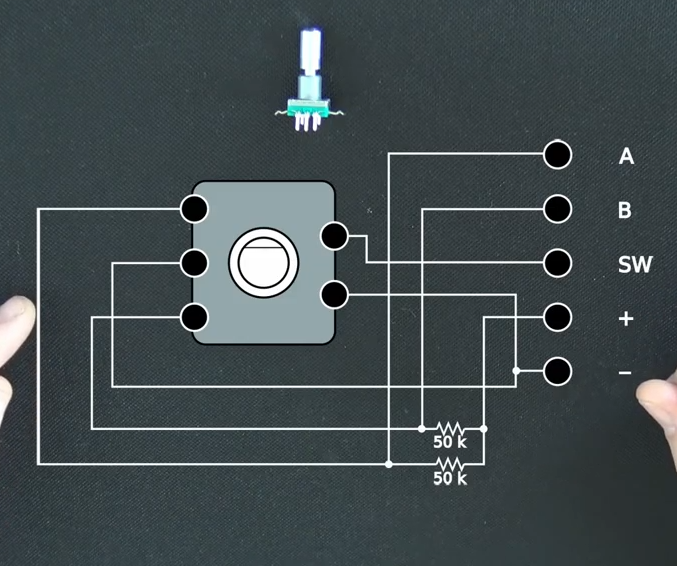
\includegraphics[width=\textwidth,height=\textheight,keepaspectratio]{rotary_encoder.PNG}
  \caption{https://www.youtube.com/watch?v=5QBeKaVrWzw}
  \label{fig:rotary_encoder}
\end{figure}

\subsection{Rotary Encoder}

When looking into my design for this controller I was going to at first have a potentiometer with a button adjacent to it to act as the submit, but I felt that this wasn't very ergonomic or practical, so I decided to look for a potentiometer with a built in button, but instead found something called a rotary encoder. I found that it is often used for GUI navigation since it rotates in 360 degrees rather than the potentiometer which is limited. This will work even better for my game since it would represent a colour wheel better. Furthermore, it also has a built in button too, so I don't have to add an extra external one, but instead an extra cable.

\begin{figure}[ht]
  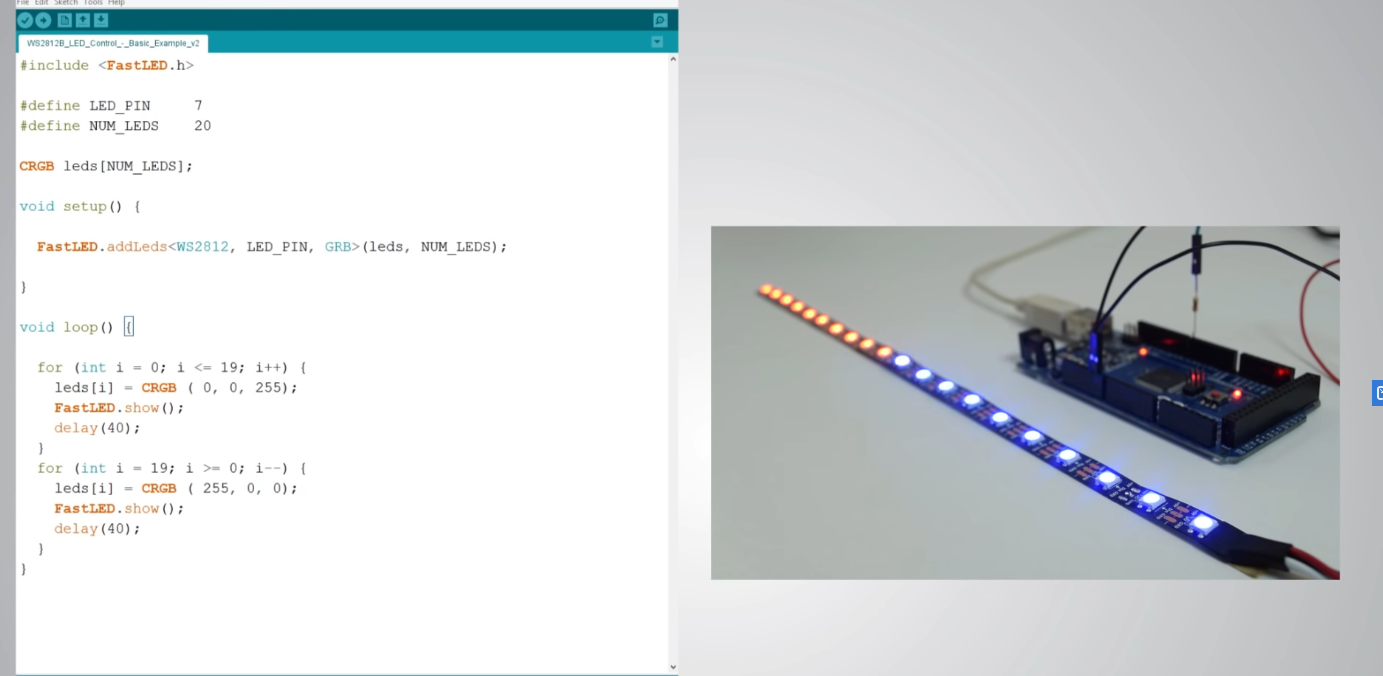
\includegraphics[width=\textwidth,height=\textheight,keepaspectratio]{led_strip.PNG}
  \caption{https://www.youtube.com/watch?v=UhYu0k2woRM}
  \label{fig:rgb_led_strip}
\end{figure}

\subsection{RGB LED Strip}

Since I want a sort of built in controller I looked at LED strips to see what I could do with them and their limitations and found that you are able to get LED strips that have each programmable LEDs with the addition of RGB which is exactly what I am aiming for. Furthermore, the video \ref{fig:rgb_led_strip} also outlines how to use a pre-made library to affect the values easily. I also checked to ensure that you are able to cut the LED strips to certain lengths and for them to still work which they do.

\begin{figure}[ht]
  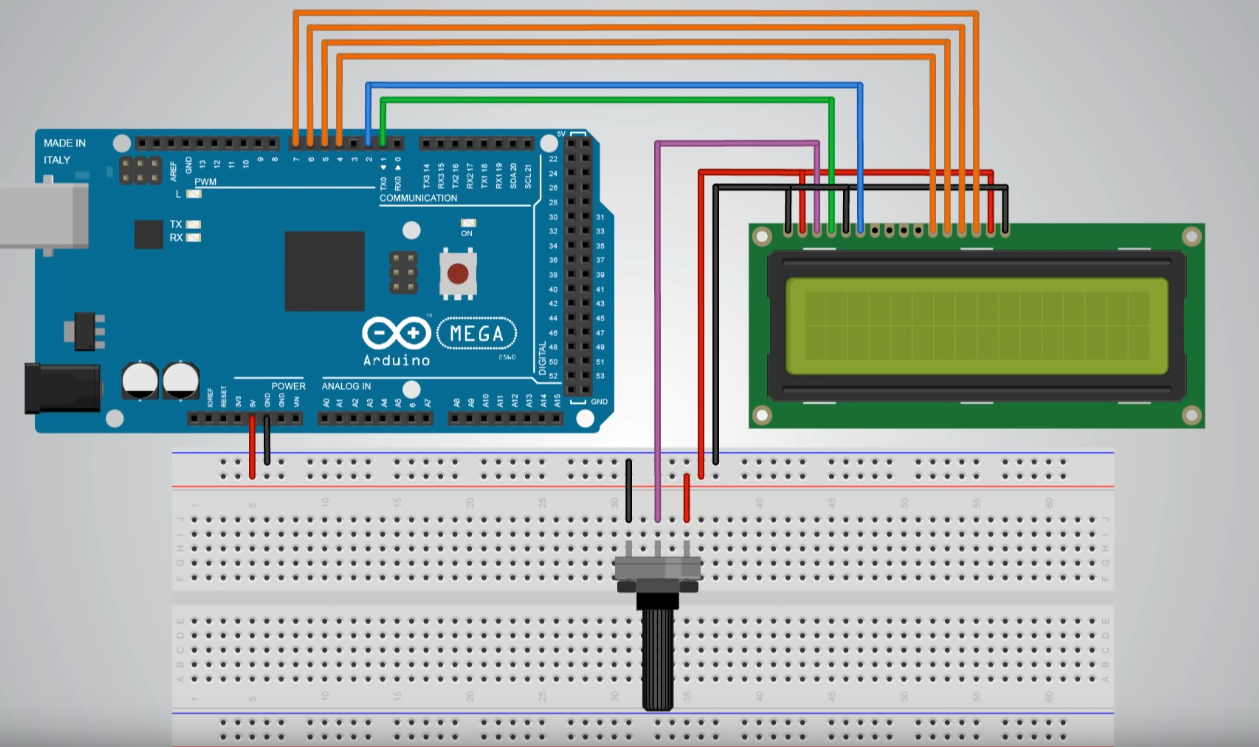
\includegraphics[width=\textwidth,height=\textheight,keepaspectratio]{lcd_display.PNG}
  \caption{https://www.youtube.com/watch?v=dZZynJLmTn8}
  \label{fig:lcd_display}
\end{figure}

\subsection{LCD Display}

I was deciding whether to use an LCD display, or a 7 segment display, but ultimately decided on the former since it provides far more customisation with what I can display on the screen and plus it has more space for characters since the segment had far less which might become problematic at higher scores for my game. Furthermore, I could also add a highscore to the LCD screen quite simply compared to the segment which would require an additional one.

\begin{figure}[ht]
  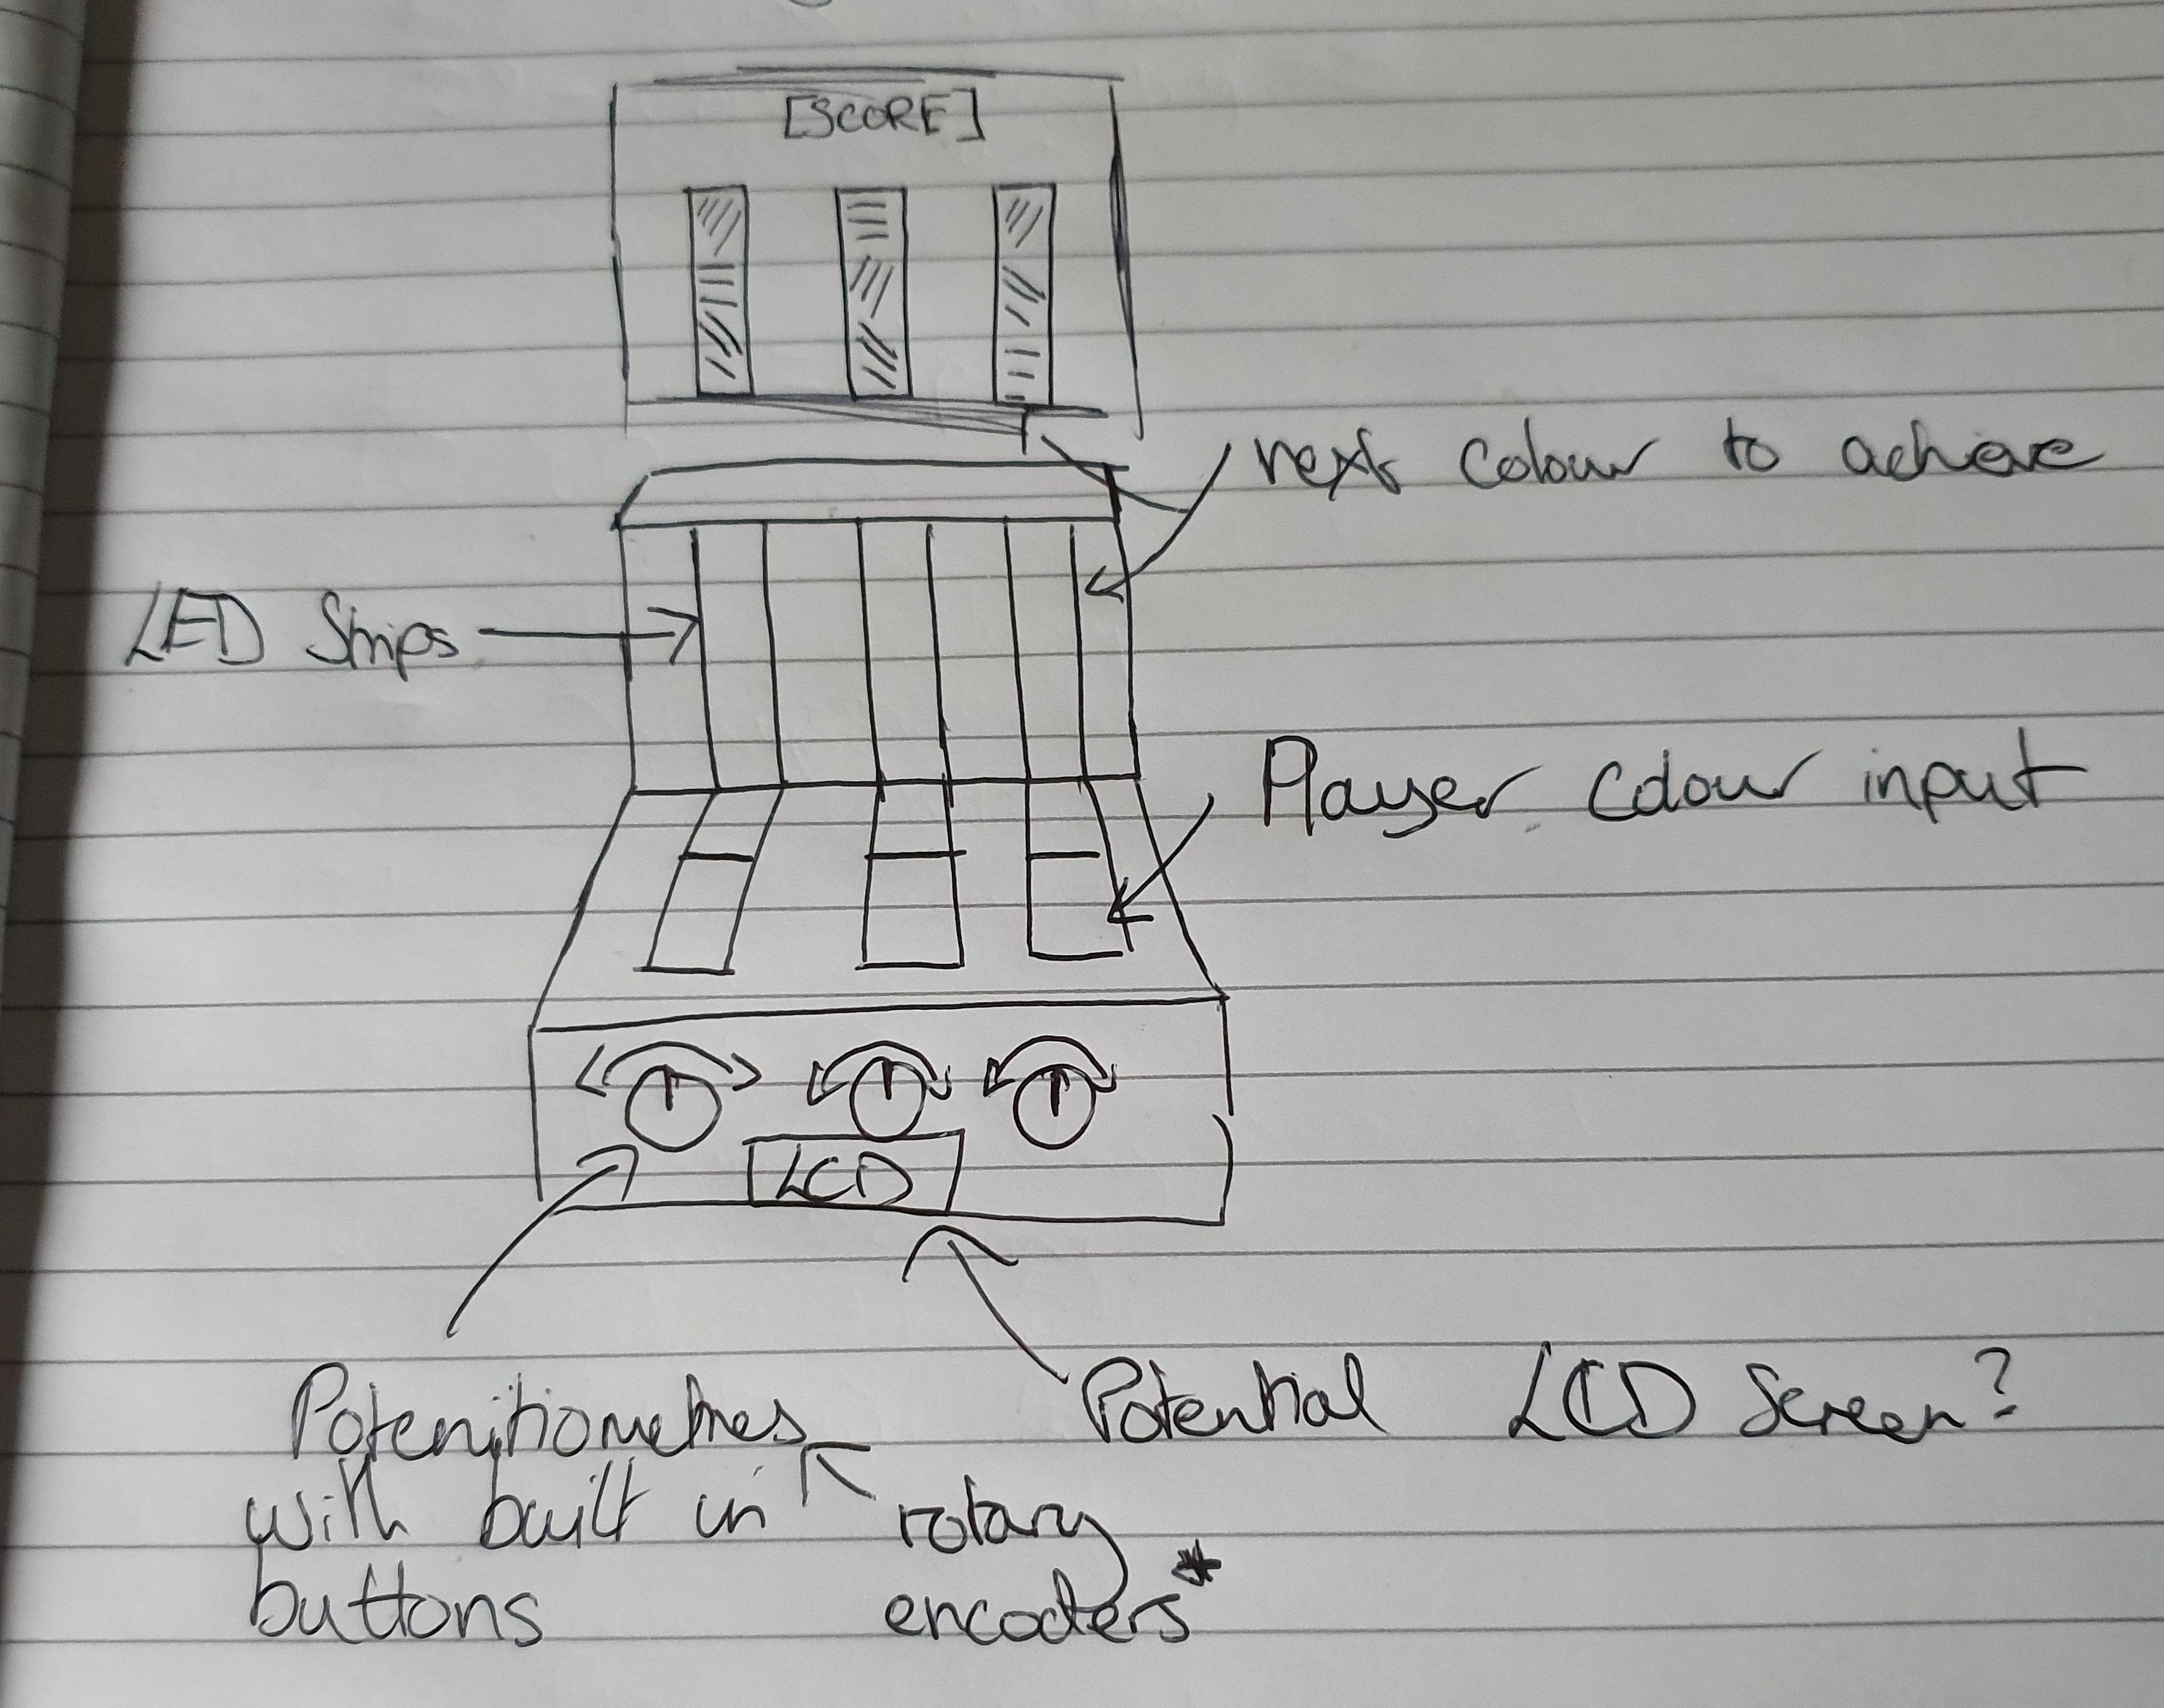
\includegraphics[width=\textwidth,height=\textheight,keepaspectratio]{controller_concept.jpg}
  \caption{Concept Art}
  \label{fig:concept}
\end{figure}

\section{Controller Design}

I intend for the controller to be completely function by itself without the use of a screen as a sort of built in controller since it will display all of the elements using RGB LED strips. It will also display the score using either an LCD screen, or a 7 Segment Display. You are then able to control the three lane inputs with rotary encoders and submit by pressing it. Although you can play it by itself I do intend on making a Unity game to go along side it which will act as an extender to see the colours further down as well as other diagnostics and general gameplay.

\section{Key Components}

\begin{itemize}
    \item Rotary Encoders x 3
    \item RGB LED Strip 5m x 1
    \item LCD Screen x 1
\end{itemize}

\section{Key User Stories}

One of the main users stories would be "As a player I want to get the correct colour to gain more score" since it is the primary objective of the game for the player.

\end{document}
